\subsection{Vista}
Le classi della vista sono state implementate utilizzando la libreria
\textbf{Swing} fornita di default dal linguaggio.\newline
Come mostrato dal \textit{class diagram} in Figura
\ref{figure:class_diagram_view} i 4 frame del gioco estendono da un'unica
classe appositamente creata per fornire una veste grafica di default:
l'\textit{AFrame}. Questo è essenzialmente un JFrame con un layout grafico
prestabilito che fornisce metodi utili per l'aggiunta e la sostituzione dei
pannelli che sono di volta in volta visualizzati. È qui che viene settato il
nome del programma come titolo della finestra, l'icona del gioco e la posizione
di comparsa sul display (al centro).\newline
Così come per i frame, tutti i pannelli estendono da un'unica classe,
l'\textit{APanel}. Anch'esso fornisce metodi per l'aggiunta dei vari oggetti che
lo popoleranno (label, aree di testo, bottoni, ecc\dots). Ogni frame mantiene al
proprio interno le istanze dei pannelli da mostrare.\newline
Un pattern molto importante e particolarmente sfruttato nell'implementazione
grafica di questo progetto è \textit{Observer}, il quale si basa su uno o più
oggetti (osservatori o observer) che vengono registrati e notificati
all'occorrenza di uno o più determinati eventi. Ogni pannello in grado di
generare eventi ha associata un'interfaccia che fornisce i metodi che
l'osservatore deve implementare per ricevere le notifiche. Dunque, ognuno dei 4
frame si comporta da osservatore nei confronti dei pannelli usati, implementando
le relative interfacce. Allo stesso modo i frame comunicano con le classi
sottostanti. Il dialogo con la vista avviene dunque in due modi:
\begin{itemize}
	\item quando dall'esterno si vuole comunicare con i frame, se ne usano i
	metodi che questi forniscono;
	\item quando invece la comunicazione parte dalla grafica, i frame usano i
	metodi forniti dalle rispettive interfacce che gli osservatori avranno il
	compito di implementare.
\end{itemize}



\subsubsection{Main Frame}
Il frame principale si compone di un unico pannello, il \textit{MainPanel}. Così
come detto in fase di progettazione (Sezione
\ref{subsubsection:progettazione_main_frame}), questo frame ha il compito di
permettere all'utente la scelta della modalità nella quale avviare il programma:
se come server (lobby) o come client (game).\newline
Per la comunicazione verso l'esterno, il MainPanel ha un'interfaccia associata
che utilizza per notificare il MainFrame alla pressione dei bottoni ``Exit'' e
``Start'' il quale, a sua volta, tramite l'observer \textit{MainFrameObserver}
notifca il \textit{Main}.



\subsubsection{Lobby Frame}
\begin{figure}[!h]
	\begin{subfigure}{.5\textwidth}
		\centering
		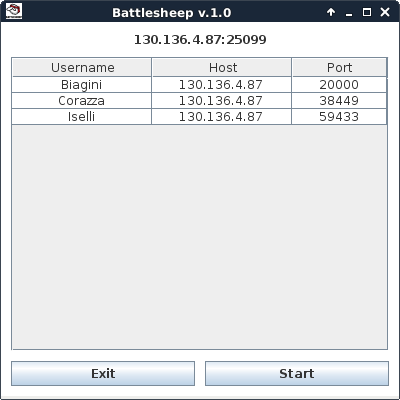
\includegraphics[scale=0.4]{core/imgs/gui/lobby_frame}
		\caption{Lobby Frame}
		\label{figure:lobby_frame}
	\end{subfigure}
	\begin{subfigure}{.5\textwidth}
		\centering
		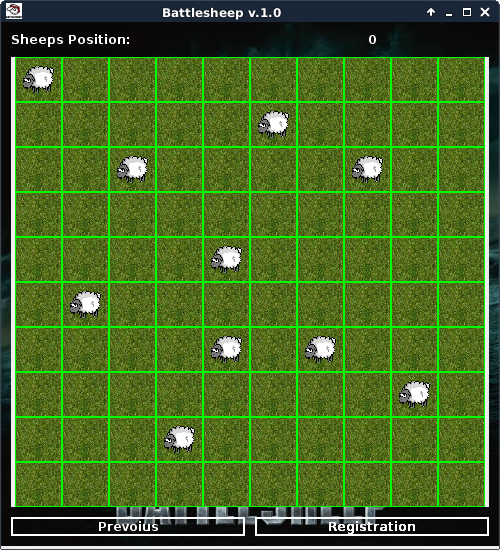
\includegraphics[scale=0.3]{core/imgs/gui/registration_frame}
		\caption{Registration Frame}
		\label{figure:registration_frame}
	\end{subfigure}
	\caption{}
\end{figure}
Il \textit{LobbyFrame} si compone di 3 pannelli così come pianificato in fase di
progettazione (Sezione~\ref{subsubsection:progettazione_lobby_frame}):
\begin{itemize}
	\item \textit{LobbyNamePanel}: è il primo pannello mostrato e peremtte agli
	utenti di scegliere il nome della stanza. Ha due bottoni, uno per l'uscita
	dal programma ed uno per l'avanzamento al pannello successivo;
	\item \textit{WaitingPanel}: è il secondo pannello che mostra una gif per
	l'attesa di connessioni da parte dei client. Ha anch'esso un bottone di
	uscita;
	\item \textit{ClientsTablePanel}: è il terzo ed ultimo pannello visibile in
	Figura~\ref{figure:lobby_frame}. Viene mostrato automaticamente non appena
	un host si connette. Ospita due bottoni: uno per l'uscita dal programma ed
	uno per l'avvio della stanza.
\end{itemize}
Quando uno dei bottoni di uscita viene premuto, il frame viene notificato dalle
funzioni usate dai pannelli per le notifiche e a sua volta propaga
l'informazione verso il prorio osservatore (\textit{Lobby}) tramite i metodi
forniti dall'intrfaccia \textit{LobbyFrameObserver}. Lo stesso comportamento
viene attuato alla pressione del bottone ``Start''. L'azione sul bottone
``Next'', invece, non viene propagata all'esterno ma serve al frame per sapere
quando visualizzare il secondo pannello.



\subsubsection{Registration Frame}
Il \textit{RegistrationFrame} si compone di 7 pannelli così come descritto in
Sezione~\ref{subsubsection:progettazione_registration_frame}.\newline
Il comportamento di questo frame è del tutto simile a quello del LobbyFrame: gli
eventi scatenati dai bottoni per l'avanzamento della registrazione (``Next'' e
``Previous'') sono usati internamente per la sostituzione dei vari pannelli
mentre, le azioni sui bottoni ``Exit'' e ``Registration'' sono propagate dal
frame verso il proprio osservatore (\textit{Battlesheep}) tramite l'interfaccia
\textit{RegistrationFrameObserver}.\newline
In Figura~\ref{figure:registration_frame} è mostrato il sesto pannello che
permette all'utente di scegliere la posizione delle proprie pecore nel campo di
gioco e di registrarsi alla lobby.



\subsubsection{Game Frame}
\begin{figure}[!h]
	\centering
	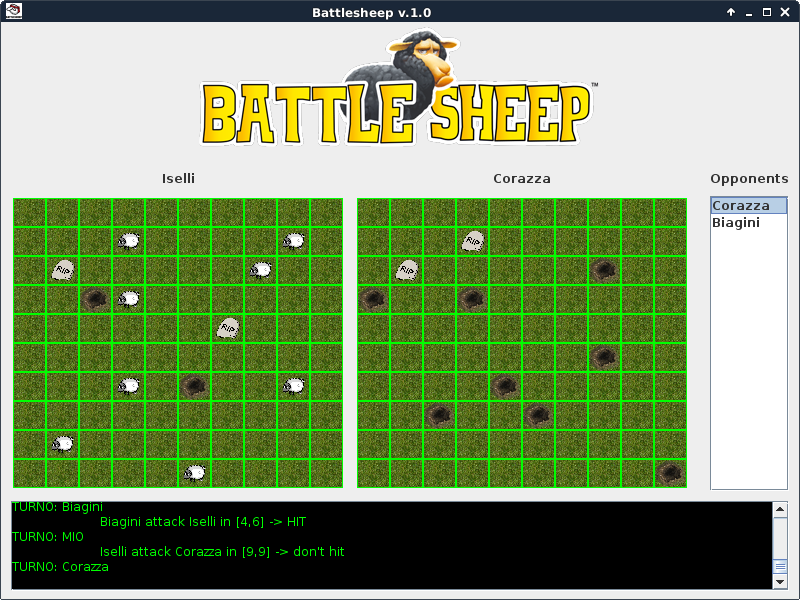
\includegraphics[scale=0.4]{core/imgs/gui/game_frame}
	\caption{Game Frame}
	\label{figure:game_frame}
\end{figure}
Il \textit{GameFrame}, mostrato in Figura~\ref{figure:game_frame}, è anch'esso
stato implementato secondo le specifiche progettuali descritte in Sezione
\ref{subsubsection:progettazione_game_frame}.\newline
La classe \textit{Battlesheep} comunica con questo frame tramite i metodi che
esso mette a disposizione principalmente per informarlo di come è tarminata la
partita per l'utente, per gli altri giocatori e su come si sono conclusi i vari
attacchi. Al contrario, il frame comunica con Battlesheep usando l'interfaccia
\textit{GameFrameObserver} per comunicare la volontà da parte dell'utente di
abbandonare il gioco o di attaccare un avversario in una daterminata posizione.
